\PassOptionsToPackage{unicode}{hyperref}
\documentclass[aspectratio=1610, 11pt]{beamer}

\usepackage{amsmath}
\usepackage{amssymb}
\usetheme{tudo}

\title{Datenstrukturen, Algorithmen und Programmierung~2}
\author[A.~Coja-Oghlan]{Amin Coja-Oghlan}
\institute[DAP2]{Lehrstuhl Informatik 2\\Fakult\"at f\"ur Informatik}

\newcommand\dist{\mathrm{dist}}
\renewcommand{\vec}[1]{\boldsymbol{#1}}
\newcommand\NULL{{\tt NULL}}
\newcommand\dd{\mathrm d}
\newcommand\eul{\mathrm e}
\newcommand\cA{\mathcal A}
\newcommand\cB{\mathcal B}
\newcommand\cC{\mathcal C}
\newcommand\cD{\mathcal D}
\newcommand\cE{\mathcal E}
\newcommand\cF{\mathcal F}
\newcommand\cG{\mathcal G}
\newcommand\cH{\mathcal H}
\newcommand\cI{\mathcal I}
\newcommand\cJ{\mathcal J}
\newcommand\cK{\mathcal K}
\newcommand\cL{\mathcal L}
\newcommand\cM{\mathcal M}
\newcommand\cN{\mathcal N}
\newcommand\cO{\mathcal O}
\newcommand\cP{\mathcal P}
\newcommand\cQ{\mathcal Q}
\newcommand\cR{\mathcal R}
\newcommand\cS{\mathcal S}
\newcommand\cT{\mathcal T}
\newcommand\cU{\mathcal U}
\newcommand\cV{\mathcal V}
\newcommand\cW{\mathcal W}
\newcommand\cX{\mathcal X}
\newcommand\cY{\mathcal Y}
\newcommand\cZ{\mathcal Z}
\newcommand\fA{\mathfrak A}
\newcommand\fB{\mathfrak B}
\newcommand\fC{\mathfrak C}
\newcommand\fD{\mathfrak D}
\newcommand\fE{\mathfrak E}
\newcommand\fF{\mathfrak F}
\newcommand\fG{\mathfrak G}
\newcommand\fH{\mathfrak H}
\newcommand\fI{\mathfrak I}
\newcommand\fJ{\mathfrak J}
\newcommand\fK{\mathfrak K}
\newcommand\fL{\mathfrak L}
\newcommand\fM{\mathfrak M}
\newcommand\fN{\mathfrak N}
\newcommand\fO{\mathfrak O}
\newcommand\fP{\mathfrak P}
\newcommand\fQ{\mathfrak Q}
\newcommand\fR{\mathfrak R}
\newcommand\fS{\mathfrak S}
\newcommand\fT{\mathfrak T}
\newcommand\fU{\mathfrak U}
\newcommand\fV{\mathfrak V}
\newcommand\fW{\mathfrak W}
\newcommand\fX{\mathfrak X}
\newcommand\fY{\mathfrak Y}
\newcommand\fZ{\mathfrak Z}
\newcommand\fa{\mathfrak a}
\newcommand\fb{\mathfrak b}
\newcommand\fc{\mathfrak c}
\newcommand\fd{\mathfrak d}
\newcommand\fe{\mathfrak e}
\newcommand\ff{\mathfrak f}
\newcommand\fg{\mathfrak g}
\newcommand\fh{\mathfrak h}
%\newcommand\fi{\mathfrak i}
\newcommand\fj{\mathfrak j}
\newcommand\fk{\mathfrak k}
\newcommand\fl{\mathfrak l}
\newcommand\fm{\mathfrak m}
\newcommand\fn{\mathfrak n}
\newcommand\fo{\mathfrak o}
\newcommand\fp{\mathfrak p}
\newcommand\fq{\mathfrak q}
\newcommand\fr{\mathfrak r}
\newcommand\fs{\mathfrak s}
\newcommand\ft{\mathfrak t}
\newcommand\fu{\mathfrak u}
\newcommand\fv{\mathfrak v}
\newcommand\fw{\mathfrak w}
\newcommand\fx{\mathfrak x}
\newcommand\fy{\mathfrak y}
\newcommand\fz{\mathfrak z}
\newcommand\vA{\vec A}
\newcommand\vB{\vec B}
\newcommand\vC{\vec C}
\newcommand\vD{\vec D}
\newcommand\vE{\vec E}
\newcommand\vF{\vec F}
\newcommand\vG{\vec G}
\newcommand\vH{\vec H}
\newcommand\vI{\vec I}
\newcommand\vJ{\vec J}
\newcommand\vK{\vec K}
\newcommand\vL{\vec L}
\newcommand\vM{\vec M}
\newcommand\vN{\vec N}
\newcommand\vO{\vec O}
\newcommand\vP{\vec P}
\newcommand\vQ{\vec Q}
\newcommand\vR{\vec R}
\newcommand\vS{\vec S}
\newcommand\vT{\vec T}
\newcommand\vU{\vec U}
\newcommand\vV{\vec V}
\newcommand\vW{\vec W}
\newcommand\vX{\vec X}
\newcommand\vY{\vec Y}
\newcommand\vZ{\vec Z}
\newcommand\va{\vec a}
\newcommand\vb{\vec b}
\newcommand\vc{\vec c}
\newcommand\vd{\vec d}
\newcommand\ve{\vec e}
\newcommand\vf{\vec f}
\newcommand\vg{\vec g}
\newcommand\vh{\vec h}
\newcommand\vi{\vec i}
\newcommand\vj{\vec j}
\newcommand\vk{\vec k}
\newcommand\vl{\vec l}
\newcommand\vm{\vec m}
\newcommand\vn{\vec n}
\newcommand\vo{\vec o}
\newcommand\vp{\vec p}
\newcommand\vq{\vec q}
\newcommand\vr{\vec r}
\newcommand\vs{\vec s}
\newcommand\vt{\vec t}
\newcommand\vu{\vec u}
\renewcommand\vv{\vec v}
\newcommand\vw{\vec w}
\newcommand\vx{\vec x}
\newcommand\vy{\vec y}
\newcommand\vz{\vec z}
\renewcommand\AA{\mathbb A}
\newcommand\NN{\mathbb N}
\newcommand\ZZ{\mathbb Z}
\newcommand\PP{\mathbb P}
\newcommand\QQ{\mathbb Q}
\newcommand\RR{\mathbb R}
\newcommand\RRpos{\mathbb R_{\geq0}}
\newcommand\QQpos{\mathbb Q_{\geq0}}
\renewcommand\SS{\mathbb S}
\newcommand\CC{\mathbb C}
\newcommand{\ord}{\mathrm{ord}}
\newcommand{\id}{\mathrm{id}}
\newcommand{\pr}{\mathrm{P}}
\newcommand{\Vol}{\mathrm{vol}}
\newcommand\norm[1]{\left\|{#1}\right\|} 
\newcommand\sign{\mathrm{sign}}
\newcommand{\eps}{\varepsilon}
\newcommand{\abs}[1]{\left|#1\right|}
\newcommand\bc[1]{\left({#1}\right)} 
\newcommand\cbc[1]{\left\{{#1}\right\}} 
\newcommand\bcfr[2]{\bc{\frac{#1}{#2}}} 
\newcommand{\bck}[1]{\left\langle{#1}\right\rangle} 
\newcommand\brk[1]{\left\lbrack{#1}\right\rbrack} 
\newcommand\scal[2]{\bck{{#1},{#2}}} 
\newcommand{\vecone}{\mathbb{1}}
\newcommand{\tensor}{\otimes}
\newcommand{\diag}{\mathrm{diag}}
\newcommand{\ggt}{\mathrm{ggT}}
\newcommand{\kgv}{\mathrm{kgV}}
\newcommand{\trans}{\top}
\newcommand{\Karonski}{Karo\'nski}
\newcommand{\Erdos}{Erd\H{o}s}
\newcommand{\Renyi}{R\'enyi}
\newcommand{\Lovasz}{Lov\'asz}
\newcommand{\Juhasz}{Juh\'asz}
\newcommand{\Bollobas}{Bollob\'as}
\newcommand{\Furedi}{F\"uredi}
\newcommand{\Komlos}{Koml\'os}
\newcommand{\Luczak}{\L uczak}
\newcommand{\Kucera}{Ku\v{c}era}
\newcommand{\Szemeredi}{Szemer\'edi}

\newcommand{\mytitle}{Binomial heaps}

\begin{document}

\frame[plain]{\titlepage}

\begin{frame}\frametitle{\mytitle}
	\begin{exampleblock}{Worum geht es?}
		\begin{itemize}
			\item der Dijkstra-Algorithmus hat quadratische Laufzeit
			\item Flaschenhals ist die Berechnung des Knotens mit minimalen Abstand
			\item mit dem binomial heap lernen wir eine erste Datenstruktur kennen, die diese Operation beschleunigt
		\end{itemize}
	\end{exampleblock}
\end{frame}

\begin{frame}\frametitle{\mytitle}
	\begin{exampleblock}{Binomial heap: \"Uberblick}
		\begin{description}
			\item[einf\"ugen:] neues Element mit gegebenen Gewicht hinzuf\"ugen
			\item[Minimum:] auffinden des Elements mit minimalen Gewicht
			\item[Minimum entnehmen:] auffinden und entfernen
			\item[Vereinigung:] zwei Heaps zu einem vereinigen
			\item[verringern:] das Gewicht eines Elements verringern
			\item[l\"oschen:] ein Element aus der Datenstruktur entfernen
		\end{description}
		\itshape Alle Operationen haben Laufzeit $O(\log n)$
	\end{exampleblock}
\end{frame}

\begin{frame}\frametitle{\mytitle}
	\hfill\includegraphics[height=20mm]{images/bintree.pdf}
	\begin{overprint}
		\onslide<1>
		\begin{exampleblock}{Binomialb\"aume}
			\begin{itemize}
				\item ein Binomialbaum ist ein geordneter, gewurzelter Baum
				\item d.h.\ ein Knoten ist als Wurzel ausgezeichnet
				\item die Kinder jedes Knotens sind geordnet
			\end{itemize}
		\end{exampleblock}
		\onslide<2>
		\begin{exampleblock}{Binomialb\"aume}
			\begin{itemize}
				\item zu jeder \alert{Ordnung} $k\geq0$ gibt es genau einen Binomialbaum, bis auf Isomorphie
				\item der Binomialbaum der Ordnung $0$ besteht nur aus einem Knoten
				\item der Baum der Ordnung $k\geq1$ entsteht aus zwei B\"aumen der Ordnung $k-1$
				\item der erste Baum wird links an die Wurzel des zweiten Baums angeh\"angt wird
			\end{itemize}
		\end{exampleblock}
		\onslide<3>
		\begin{exampleblock}{Binomialb\"aume}
			\begin{itemize}
				\item im Baum der Ordnung $k$ h\"angt an der Wurzel also jeweils ein Baum der Ordnung $0,1,\ldots,k-1$
			\end{itemize}
		\end{exampleblock}
		\onslide<4>
		\begin{block}{Lemma}
			Der Binomialbaum $B_k$ der Ordnung $k\geq0$ hat folgende Eigenschaften
			\begin{itemize}
				\item die Zahl der Knoten ist $2^k$
				\item die H\"ohe des Baums ist $k$
				\item es gibt genau $\binom kh$ Knoten auf Tiefe $h$ f\"ur $h=0,\ldots,k$
				\item die Wurzel hat Grad $k=\Delta(B_k)$
			\end{itemize}
			\itshape Die Tiefe eines Knotens ist definiert als der Abstand von der Wurzel.
		\end{block}
		\onslide<5>
		\begin{exampleblock}{Beweis}
			\begin{itemize}
				\item Induktion nach $k$
				\item im Fall $k=0$ gelten die gew\"unschten Eigenschaften
				\item f\"ur $k>0$ folgen die Behauptungen zu Knotenzahl, H\"ohe und Grad der Wurzel unmittelbar aus der Induktionsvoraussetzung
				\item die Zahl der Knoten auf Tiefe $0\leq h\leq k$ berechnet sich nach Induktion zu
					$$\binom kh+\binom k{h-1}=\binom{k+1}h$$
				\item es gibt genau einen Knoten auf Tiefe $k+1$
			\end{itemize}
		\end{exampleblock}
	\end{overprint}
\end{frame}

\begin{frame}\frametitle{\mytitle}
	\hfill\includegraphics[height=20mm]{images/binheap.pdf}
	\begin{overprint}
		\onslide<1>
		\begin{exampleblock}{Binomial heap: Konstruktion}
			\begin{itemize}
				\item ein binomial heap ist eine verkettete Liste von Binomialb\"aumen 
				\item genauer sei $n\ge1$ eine ganze Zahl mit Bin\"ardarstellung $n=\sum_{j=0}^\ell b_j2^j$ mit $b_j\in\{0,1\},\ b_\ell=1$
				\item dann enth\"alt der binomial heap der Ordnung $n$ genau $b_j$ Binomialb\"aume der Ordnung $j$ f\"ur $j=0,\ldots,\ell$
			\end{itemize}
		\end{exampleblock}
		\onslide<2>
		\begin{exampleblock}{Binomial heap: Konstruktion}
			\begin{itemize}
				\item diese Binomialb\"aume bilde eine der Ordnung nach aufsteigend geordnete verkettete Liste
				\item jeder einzelne Binomialbaum besteht aus einem Zeiger auf die Wurzel 
				\item jeder Knoten ausser der Wurzel verf\"ugt \"uber einen Zeiger auf seinen Elternknoten
				\item ferner besitzt jeder Knoten einen Zeiger auf den n\"achsten Geschwisterknoten
			\end{itemize}
		\end{exampleblock}
		\onslide<3>
		\begin{exampleblock}{Binomial heap: Konstruktion}
			\begin{itemize}
				\item der binomial heap besteht also aus $O(\log n)$ B\"aumen
				\item die maximale Tiefe dieser B\"aume ist $O(\log n)$
			\end{itemize}
		\end{exampleblock}
		\onslide<4>
		\begin{exampleblock}{Binomial heap: Konstruktion}
			\begin{itemize}
				\item innerhalb jedes Baumes ist das Gewicht des Elternknotens immer kleiner oder gleich dem Gewicht jedes Kindknotens
				\item insbesondere hat der Wurzelknoten das geringste Gewicht
				\item die Gewichte der Wurzelknoten im binomial heap sind nicht notwendigerweise geordnet
			\end{itemize}
		\end{exampleblock}
	\end{overprint}
\end{frame}

\begin{frame}\frametitle{\mytitle}
	\hfill\includegraphics[height=20mm]{images/binheap.pdf}
	\begin{overprint}
		\onslide<1>
		\begin{exampleblock}{Binomial heap: Minimum finden}
			\begin{itemize}
				\item das Element minimalen Gewichts finden wir, indem wir einfach die Wurzelknoten der B\"aume des binomial heap durchsuchen
				\item das funktioniert, weil in jedem einzelen binomial tree die Wurzel das Element minimalen Gewichts ist
				\item Zeitbedarf: $O(\log n)$
			\end{itemize}
		\end{exampleblock}
		\onslide<2>
		\begin{exampleblock}{Binomial heap: Vereinigung}
			\begin{itemize}
				\item um zwei binomial heaps $B_1,B_2$ zu vereinigen, f\"ugen wir zun\"achst die Listen der Binomialb\"aume zusammen
				\item beim Zusammenf\"ugen wird die Ordnung beibehalten
				\item es treten also zu jeder Ordnung $j$ h\"ochsts zwei B\"aume der Ordnung $j$ auf
				\item beim Vereinigungsprozess kann ein dritter Baum einer gegebenen Ordnung entstehen
			\end{itemize}
		\end{exampleblock}
		\onslide<3>
		\begin{exampleblock}{Binomial heap: Vereinigung}
			\begin{itemize}
				\item anschlie\ss end gehen wir die vereinige Liste der B\"aume durch
				\item wenn von einer Ordnung genau zwei B\"aume vorkommen, vereinigen wir sie
				\item wenn von einer Ordnung drei B\"aume vorkommen, behalten wir den ersten bei und vereinigen die beiden anderen
			\end{itemize}
		\end{exampleblock}
		\onslide<4>
		\begin{exampleblock}{Binomial heap: Vereinigung}
			\begin{itemize}
				\item dabei stellen wir sicher, da\ss\ die Wurzel das Element geringsten Gewichtes bleibt
				\item die Laufzeit f\"ur den Vereinigungsprozess liegt bei $O(\log n)$
			\end{itemize}
		\end{exampleblock}
		\onslide<5>
		\begin{exampleblock}{Binomial heap: Element einf\"ugen}
			\begin{itemize}
				\item zum Einf\"ugen eines neuen Elementes in eine binomial heap $H$ legen wir einen binomial heap $H'$ der Ordnung $0$ an, der \emph{nur} das neue Element enth\"alt
				\item dann bilden wir die Vereinigung von $H$ und $H'$
				\item Laufzeit: $O(\log n)$
			\end{itemize}
		\end{exampleblock}
		\onslide<6>
		\begin{exampleblock}{Binomial heap: Minimum entnehmen}
			\begin{itemize}
				\item finde das Element $x$ minimalen Gewichts in $H$
				\item dieses Element ist Wurzel eines Binomialbaums $T$
				\item bilde einen neuen binomial heap $H'$, dessen Elemente die Kinder von $T$ (in umgekehrter Reihenfolge) sind
				\item vereinige $H'$ mit dem binomial heap $H''=H-T$ 
				\item Laufzeit: $O(\log n)$
			\end{itemize}
		\end{exampleblock}
		\onslide<7>
		\begin{exampleblock}{Binomial heap: Gewicht verringern}
			\begin{itemize}
				\item um das Gewicht eines Elements $x$ zu verringern, m\"ussen nur die Elemente des Baums, dem $x$ angeh\"ort, neu angeordnet werden
				\item genauer lassen wir $x$ in Richtung Wurzel aufsteigen, bis alle Kinder von $x$ mindestens das Gewicht von $x$ haben
				\item Laufzeit $O(\log n)$, weil die Tiefe des Baums $O(\log n)$ ist
			\end{itemize}
		\end{exampleblock}
		\onslide<8>
		\begin{exampleblock}{Binomial heap: l\"oschen}
			\begin{itemize}
				\item setze das Gewicht des zu l\"oschenden Elements auf $-\infty$
				\item anschlie\ss end entfere das Minimum
				\item Laufzeit: $O(\log n)$
			\end{itemize}
		\end{exampleblock}
	\end{overprint}
\end{frame}

\begin{frame}\frametitle{\mytitle}
	\begin{overprint}
		\onslide<1>
		\begin{exampleblock}{Anwendung auf Dijkstra}
			K\"urzeste Pfade in einem Graphen $G=(V,E)$
			\begin{itemize}
				\item naiver Dijkstra hatte Laufzeit $O(|V|^2)$
				\item mit binomial heaps ist die Laufzeit $O(|E|\log|V|)$
				\item besser als naiver Dijkstra in ``d\"unnen'' Graphen
			\end{itemize}
		\end{exampleblock}
	\end{overprint}
\end{frame}

\begin{frame}\frametitle{\mytitle}
	\begin{overprint}
		\onslide<1>
		\begin{exampleblock}{Zusammenfassung}
			\begin{itemize}
				\item binomial heaps sind geeignet, um gewichtete Elemente zu speichern, wenn man an dem Element minimalen Gewichts interessiert ist
				\item Laufzeit aller Operationen ist $O(\log n)$
				\item \emph{Anwendung:} Dijkstra
			\end{itemize}
		\end{exampleblock}
	\end{overprint}
\end{frame}

\end{document}
